\documentclass[12pt]{article}
\date{March 30, 2020}
\usepackage{pgf-pie}
\usepackage{pgfplots}
\usepackage{pgfplotstable}
\usetikzlibrary{patterns}
\usepackage[section]{placeins}
\usepackage[utf8]{inputenc}

\begin{document}


\clearpage{}
\section{รหัสผู้ให้ข้อมูล}

\label{sec:250}


\begin{figure}[h!]
    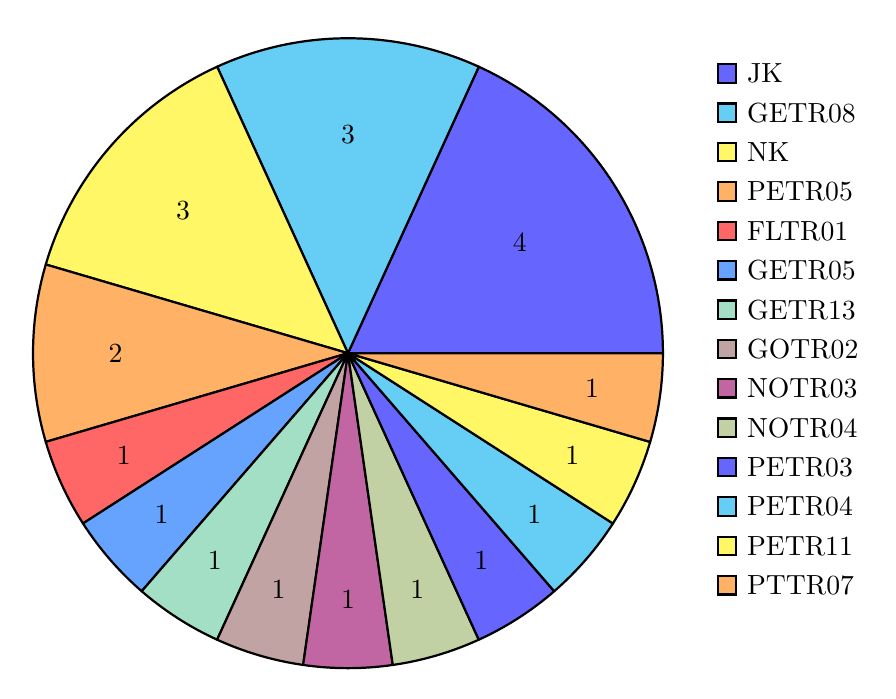
\begin{tikzpicture}
        \pie[radius=4,sum=auto,text=legend]{
            4/JK,
            3/GETR08,
            3/NK,
            2/PETR05,
            1/FLTR01,
            1/GETR05,
            1/GETR13,
            1/GOTR02,
            1/NOTR03,
            1/NOTR04,
            1/PETR03,
            1/PETR04,
            1/PETR11,
            1/PTTR07
        }
    \end{tikzpicture}
    \caption{\label{figure:q250-1}Repartition of answers for the question 'รหัสผู้ให้ข้อมูล'.}
\end{figure}



\clearpage{}
\section{ท่านมีความลำบากในการออกเสียงคำบางคำ}

\label{sec:130}


\begin{figure}[h!]
    \begin{tikzpicture}
        \pie[radius=4,sum=auto,text=legend]{
            14/2-เปนบางครง,
            12/0-ไมเคย,
            5/Left blank,
            2/1-แทบจะไมเคย,
            1/3-คอนขางบอย,
            1/4-บอยครงมาก
        }
    \end{tikzpicture}
    \caption{\label{figure:q130-1}Repartition of answers for the question 'ท่านมีความลำบากในการออกเสียงคำบางคำ'.}
\end{figure}



\clearpage{}
\section{ท่านรู้สึกว่ารสชาติอาหารแย่ลง}

\label{sec:131}


\begin{figure}[h!]
    \begin{tikzpicture}
        \pie[radius=4,sum=auto,text=legend]{
            14/2-เปนบางครง,
            10/0-ไมเคย,
            8/1-แทบจะไมเคย,
            2/3-คอนขางบอย,
            1/Left blank
        }
    \end{tikzpicture}
    \caption{\label{figure:q131-1}Repartition of answers for the question 'ท่านรู้สึกว่ารสชาติอาหารแย่ลง'.}
\end{figure}



\clearpage{}
\section{ท่านมีอาการปวด เสียว ในช่องปาก}

\label{sec:132}


\begin{figure}[h!]
    \begin{tikzpicture}
        \pie[radius=4,sum=auto,text=legend]{
            20/2-เปนบางครง,
            5/4-บอยครงมาก,
            4/1-แทบจะไมเคย,
            3/3-คอนขางบอย,
            2/0-ไมเคย,
            1/Left blank
        }
    \end{tikzpicture}
    \caption{\label{figure:q132-1}Repartition of answers for the question 'ท่านมีอาการปวด เสียว ในช่องปาก'.}
\end{figure}



\clearpage{}
\section{ท่านลำบาก/ไม่สุขสบายในการรับประทานอาหาร}

\label{sec:133}


\begin{figure}[h!]
    \begin{tikzpicture}
        \pie[radius=4,sum=auto,text=legend]{
            16/2-เปนบางครง,
            6/0-ไมเคย,
            6/3-คอนขางบอย,
            5/1-แทบจะไมเคย,
            1/Left blank,
            1/4-บอยครงมาก
        }
    \end{tikzpicture}
    \caption{\label{figure:q133-1}Repartition of answers for the question 'ท่านลำบาก/ไม่สุขสบายในการรับประทานอาหาร'.}
\end{figure}



\clearpage{}
\section{ท่านรู้สึกประหม่า/อาย จากปัญหาในช่องปาก}

\label{sec:134}


\begin{figure}[h!]
    \begin{tikzpicture}
        \pie[radius=4,sum=auto,text=legend]{
            18/2-เปนบางครง,
            8/1-แทบจะไมเคย,
            6/0-ไมเคย,
            2/3-คอนขางบอย,
            1/Left blank
        }
    \end{tikzpicture}
    \caption{\label{figure:q134-1}Repartition of answers for the question 'ท่านรู้สึกประหม่า/อาย จากปัญหาในช่องปาก'.}
\end{figure}



\clearpage{}
\section{ท่านเครียดจากปัญหาในช่องปาก}

\label{sec:135}


\begin{figure}[h!]
    \begin{tikzpicture}
        \pie[radius=4,sum=auto,text=legend]{
            18/2-เปนบางครง,
            8/1-แทบจะไมเคย,
            6/0-ไมเคย,
            2/3-คอนขางบอย,
            1/Left blank
        }
    \end{tikzpicture}
    \caption{\label{figure:q135-1}Repartition of answers for the question 'ท่านเครียดจากปัญหาในช่องปาก'.}
\end{figure}



\clearpage{}
\section{ท่านรู้สึกไม่พอใจกับการรับประทานอาหารเนื่องจากปัญหาในช่องปาก}

\label{sec:136}


\begin{figure}[h!]
    \begin{tikzpicture}
        \pie[radius=4,sum=auto,text=legend]{
            12/2-เปนบางครง,
            8/3-คอนขางบอย,
            7/1-แทบจะไมเคย,
            6/0-ไมเคย,
            2/Left blank
        }
    \end{tikzpicture}
    \caption{\label{figure:q136-1}Repartition of answers for the question 'ท่านรู้สึกไม่พอใจกับการรับประทานอาหารเนื่องจากปัญหาในช่องปาก'.}
\end{figure}



\clearpage{}
\section{ท่านต้องหยุดการรับประทานอาหารกลางคัน จากปัญหาในช่องปาก}

\label{sec:137}


\begin{figure}[h!]
    \begin{tikzpicture}
        \pie[radius=4,sum=auto,text=legend]{
            14/0-ไมเคย,
            11/2-เปนบางครง,
            6/1-แทบจะไมเคย,
            2/Left blank,
            1/3-คอนขางบอย,
            1/4-บอยครงมาก
        }
    \end{tikzpicture}
    \caption{\label{figure:q137-1}Repartition of answers for the question 'ท่านต้องหยุดการรับประทานอาหารกลางคัน จากปัญหาในช่องปาก'.}
\end{figure}



\clearpage{}
\section{ท่านรู้สึกปัญหาในช่องปากทำให้ท่านรู้สึกไม่ผ่อนคลาย}

\label{sec:138}


\begin{figure}[h!]
    \begin{tikzpicture}
        \pie[radius=4,sum=auto,text=legend]{
            14/1-แทบจะไมเคย,
            9/0-ไมเคย,
            8/2-เปนบางครง,
            2/Left blank,
            2/3-คอนขางบอย
        }
    \end{tikzpicture}
    \caption{\label{figure:q138-1}Repartition of answers for the question 'ท่านรู้สึกปัญหาในช่องปากทำให้ท่านรู้สึกไม่ผ่อนคลาย'.}
\end{figure}



\clearpage{}
\section{ท่านรู้สึกเบื่อหน่ายกับปัญหาในช่องปาก}

\label{sec:139}


\begin{figure}[h!]
    \begin{tikzpicture}
        \pie[radius=4,sum=auto,text=legend]{
            12/0-ไมเคย,
            12/2-เปนบางครง,
            4/1-แทบจะไมเคย,
            4/3-คอนขางบอย,
            2/Left blank,
            1/4-บอยครงมาก
        }
    \end{tikzpicture}
    \caption{\label{figure:q139-1}Repartition of answers for the question 'ท่านรู้สึกเบื่อหน่ายกับปัญหาในช่องปาก'.}
\end{figure}



\clearpage{}
\section{ท่านรู้สึกหงุดหงิดคนรอบข้างจากปัญหาในช่องปากของท่าน}

\label{sec:140}


\begin{figure}[h!]
    \begin{tikzpicture}
        \pie[radius=4,sum=auto,text=legend]{
            14/2-เปนบางครง,
            12/0-ไมเคย,
            7/1-แทบจะไมเคย,
            2/Left blank
        }
    \end{tikzpicture}
    \caption{\label{figure:q140-1}Repartition of answers for the question 'ท่านรู้สึกหงุดหงิดคนรอบข้างจากปัญหาในช่องปากของท่าน'.}
\end{figure}



\clearpage{}
\section{ท่านมีความลำบากในการทำงานประจำจากปัญหาในช่องปาก}

\label{sec:141}


\begin{figure}[h!]
    \begin{tikzpicture}
        \pie[radius=4,sum=auto,text=legend]{
            14/1-แทบจะไมเคย,
            12/0-ไมเคย,
            6/2-เปนบางครง,
            3/Left blank
        }
    \end{tikzpicture}
    \caption{\label{figure:q141-1}Repartition of answers for the question 'ท่านมีความลำบากในการทำงานประจำจากปัญหาในช่องปาก'.}
\end{figure}



\clearpage{}
\section{ท่านพึงพอใจในชีวิตท่านโดยทั่วไปน้อยลงจากปัญหาในช่องปาก}

\label{sec:142}


\begin{figure}[h!]
    \begin{tikzpicture}
        \pie[radius=4,sum=auto,text=legend]{
            16/1-แทบจะไมเคย,
            9/0-ไมเคย,
            7/2-เปนบางครง,
            3/Left blank
        }
    \end{tikzpicture}
    \caption{\label{figure:q142-1}Repartition of answers for the question 'ท่านพึงพอใจในชีวิตท่านโดยทั่วไปน้อยลงจากปัญหาในช่องปาก'.}
\end{figure}



\clearpage{}
\section{ท่านไม่สามารถทำงานได้เต็มประสิทธิภาพจากปัญหาในช่องปาก}

\label{sec:143}


\begin{figure}[h!]
    \begin{tikzpicture}
        \pie[radius=4,sum=auto,text=legend]{
            15/1-แทบจะไมเคย,
            10/0-ไมเคย,
            8/2-เปนบางครง,
            2/Left blank
        }
    \end{tikzpicture}
    \caption{\label{figure:q143-1}Repartition of answers for the question 'ท่านไม่สามารถทำงานได้เต็มประสิทธิภาพจากปัญหาในช่องปาก'.}
\end{figure}



\end{document}
